\section{Raft} \label{sec:raft}

It is not our intention to plagiarize Ongaro and Ousterhout's excellent work "In Search of an Understandable Consensus Algorithm" \cite{raft} by presenting the Raft algorithm's specifications. Instead, we will discuss how we interpreted and implemented it to mold it into our own use case

The algorithm uses three types of nodes, namely \textit{leader}, \textit{follower} and \textit{candidate}, and revolves around three core functionalities: leader election, log replication and cluster membership change. Log compaction is also mentioned, while a byzantine fault tolerant variant is never explored by the original authors.

One last component, instrumental to the functioning of the algorithm, is the \textit{term}: everything happens in a certain term, which divides time logically and increments every election. 

Our Raft class directly extends \textit{simpleXMLRPCServer} from XML-RPC module, as shown at code \ref{code:raft}.

Lastly, to fire off non-blocking concurrent RPCs on the cluster, we leverage the \textit{concurrent.futures} module using \textit{ThreadPoolExecutor}. To avoid having to keep creating and destroying pools every time a server needs to communicate with the cluster, we embedded a finite amount of workers as class attributes (code \ref{code:threadPool}).

\begin{python}[label={code:raft}, caption={Class Raft definition}]
class Raft(SimpleXMLRPCServer):
    def __init__(self, 
                 addr: tuple[str, int],
                 allow_none: bool = True,
                 # ...
                 last_index_on_server: list[tuple[int, int]] | None = None
                 ):
        SimpleXMLRPCServer.__init__(self, addr=addr, allow_none=allow_none)
\end{python}

\begin{python}[label={code:threadPool}, caption={ThreadPoolExecutor workers}]
class Raft(SimpleXMLRPCServer):
    def __init__(self, 
                 # ...
                 )
        # start executors pool
        self.executor = concurrent.futures.ThreadPoolExecutor(max_workers=len(self.cluster))
\end{python}

\subsection{Node Types} \label{sec:nodes}

There are three types of node, namely leader, follower and candidate (code \ref{code:nodeModes}). In this section we are going to show their characteristics and similarities. Note that all nodes have a timer: it is randomized for each of them and has been implemented by extending \textit{threading.Timer}, thus making it thread-safe (code \ref{code:loopingTimer})

\begin{python}[label={code:nodeModes}, caption={Node modes}]
class Raft(SimpleXMLRPCServer):
    class Mode(Enum):
        LEADER = 1
        CANDIDATE = 2
        FOLLOWER = 3
                
    def __init__(self, 
                 # ...
                 mode: Mode = Mode.FOLLOWER,
                 )
\end{python}

\begin{python}[label={code:loopingTimer}, caption={Threadsafe looping timer}]
class LoopTimer(Timer):
    def __init__(self, interval, function, args=None, kwawrgs=None):
        Timer.__init__(self, interval, function, args, kwawrgs)
        self.was_reset : bool = False
    # ...

class Raft(SimpleXMLRPCServer):
    def __init__(self, 
                 # ...
                 )
        # start timer
        self.timer = LoopTimer(timeout, self.on_timeout)
        self.timer.start()
\end{python}

\subsubsection{Leader Node}

The algorithm revolves around one leader node, whose job is to synchronize all servers' logs to ensure data consistency. It does so by replicating its own log on all followers (the non-leader nodes) by sending new or, if needed, old entries via remote procedure calls. 

To make sure all nodes believe the leader's alive, it sends periodically (every 150-300ms) an empty remote procedure call called \textit{heartbeat}

\subsubsection{Follower Node}

All nodes, except for the leader, are classified as followers. They are not allowed to replicate their own log, and when they receive any request they have to forward it to the leader.

To make sure the cluster never remains without a leader, every follower have an election timeout (between 150ms and 300ms) which resets every time an RPC from the leader gets received. When times out, the follower change its state to \textit{candidate}, increment its current term and starts a leader election. 

Followers become candidates in another scenario: whenever they receive an entry from the leader, they compare it with their own last log entry. If the leader's term is smaller the \textit{append entry} is rejected and a new election is started. 

\subsubsection{Candidate Node}

When a follower's election timeout times out, it becomes a candidate, increment its own term and starts an election. It votes for itself and then wait for either of two outcomes: wins, thus becoming a new leader, or looses (ether another leader gets elected or the old one manifest itself) thus reverting back to being a follower.

\subsection{Log}

As stated, the leader's job is to accept requests (in our specific case they are player inputs) and then forward them to the followers. Let's talk about the structure of the log. 

The log is basically a \textit{list} (or an \textit{array}) of entries, where \textit{entry} is an element that encapsulates data (like an integer or a string), has an index (unique for each entry) and the term of its creation (figure \ref{fig:logStructure}). We defined entries as \textit{Data Classes} \footnote{Data Classes module provides a decorator and functions for automatically adding generated special methods to user-defined classes: \url{https://docs.python.org/3/library/dataclasses.html}} (decorators that simulate C's structures) as can be seen in code \ref{code:entry}.

\begin{python}[label={code:entry}, caption={Dataclass Entry definition}]
@dataclass
class Entry:
    term: int
    index: int
    command: str 
\end{python}

\begin{figure}[h]
  \centering
  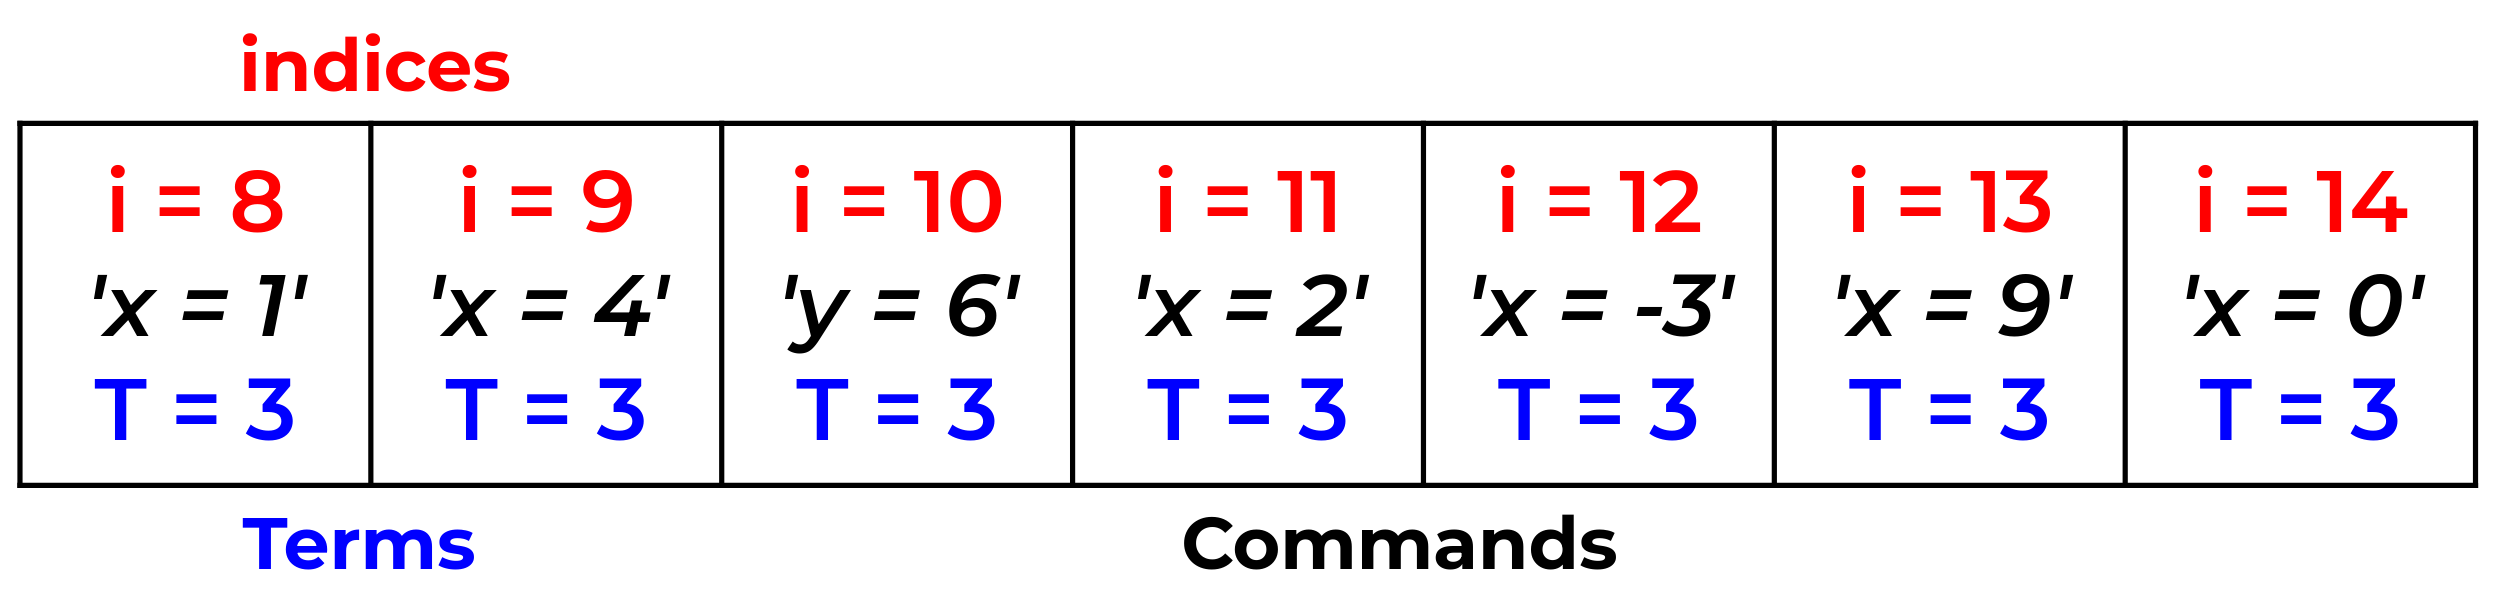
\includegraphics[width=.8\linewidth]{images/logStructure.png}
  
  \caption{Raft's log is fundamentally an array made of entries.}
  \Description{An array, thus a list of consecutive elements, each of which is an entry with its own index, term and data.}
  \label{fig:logStructure}
\end{figure}

\subsection{Log Replication and Overwriting}

All log propagation revolves around one core remote procedure call named \textit{append\_entries\_rpc}, which the leader calls on a list of server proxies that connects it to the followers, which in turn call on a proxy of the leader. It must be registered in the server to be callable, as can be seen in listing \ref{code:registerFunction}.

\begin{python}[label={code:registerFunction}, caption={Register, thus making it callable, the remote procedure call \textit{append\_entries\_rpc}}]
def handle_server():                                    # enclose server in a callable function
    with Raft(...) as server:                           # creates SimpleXMLRPCSever
        def append_entries_rpc(entries, term, commit_index, all_log):
            # ...
        server.register_function(append_entries_rpc)    # makes function callable on the other side
        server.serve_forever()                          # keeps server alive 
\end{python}

\subsubsection{Leader Propagates Entries} \label{sec:leaderSends}

The leader (each server as a matter of fact) periodically checks whether there are new commands to propagate (always stored in queue \textit{pygame\_commands}), by overriding \textit{SimpleXMLRPCServer}'s method \textit{service\_actions} (listing \ref{code:addCommands}, more details in section \ref{sec:raftian}).

Then, translates them into entries by giving each of them the current term and a log index that starts from $lastLogEntry(index) + 1$ and increases by one for each entry. To give an example: if $lastLogEntry(index) = 7$ and we have three new commands, their indexes will respectively be eight (8), nine (9) and ten (10). The translation can be seen at listing \ref{code:translateCommands}

At this point it propagates \textit{new\_entries} to the whole cluster, updating the commit index (necessary for applying log to state) as soon as propagations are successful on at least half of the cluster, like so: $commitIndex = lastNewEntry(index)$. 

What happens if the \textit{append entries} gets rejected? The leader adds to \textit{new\_entries} its own last log entry: $new\_entries = lastLogEntry + new\_entries$ (figure \ref{fig:newEntries}). Then repeats the propagation procedure, for each reject a new \textit{last log entry} gets added, progressively traversing the log backwards. If, at a certain point, $new\_entries == allLog + new\_entries$ (i.e., all leader's log gets propagated) the flag \textit{all\_log} is set to \textit{True}. 

Since every server may reject or accept different sets of entries, depending on their own local log, every propagation must be "local" for each follower. 

The flow of execution for the log propagation is: \textit{Raft: service\_actions} \faArrowRight\ \textit{Raft: propagate\_entries} \faArrowRight\ \textit{propagate\_entries} \textit{:encapsulates\_proxy:} \textit{append\_entries\_rpc}. The last one gets called as many times as needed on every single follower.

Of course, all propagation happens concurrently using a \textit{ThreadPoolExecutor}, and the code for entries propagation (leader's side) can be seen at listing \ref{code:leaderPropagateEntries}.

\begin{figure}[h]
  \centering
  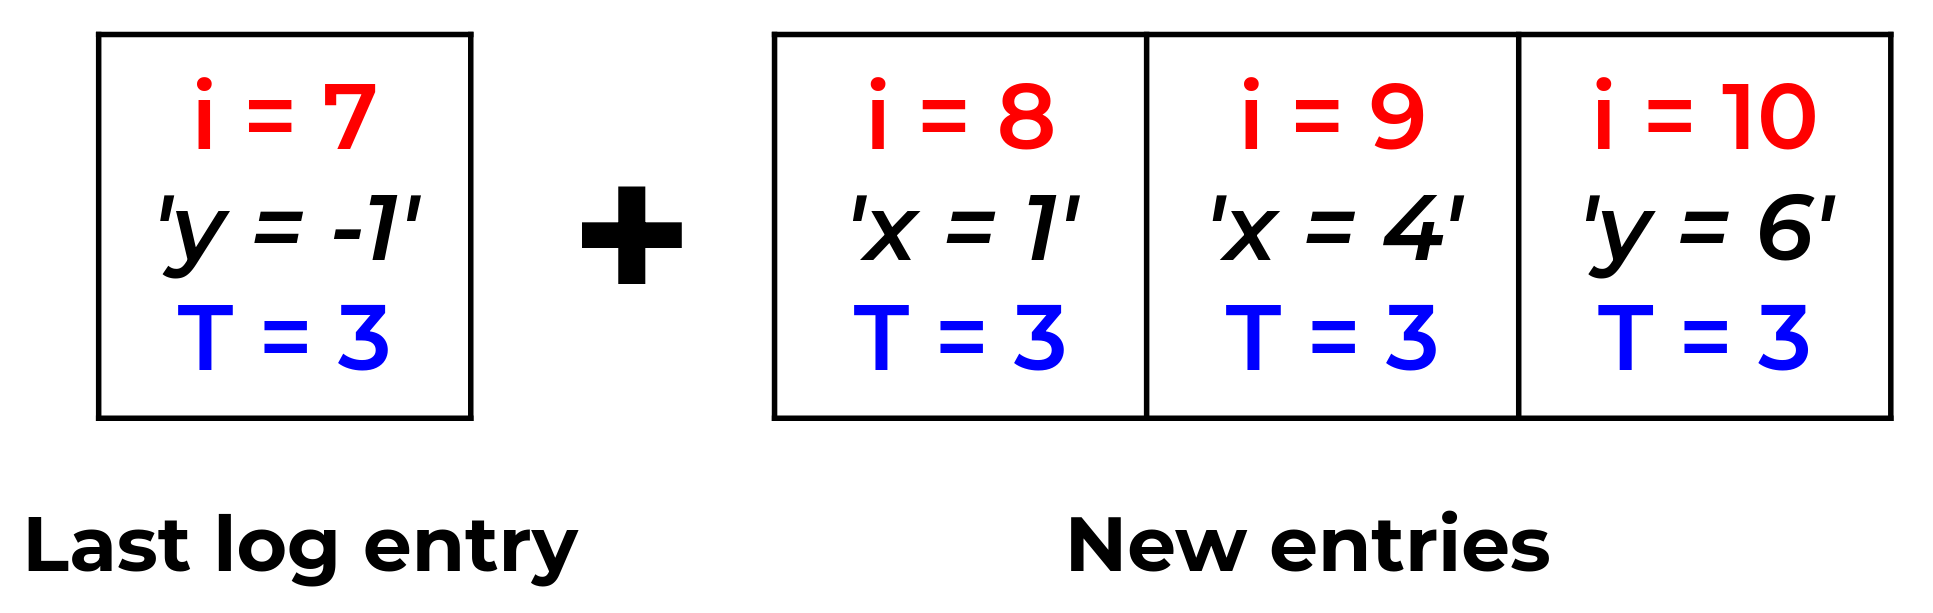
\includegraphics[width=.8\linewidth]{images/newEntries.png}
  
  \caption{New entries with the last log's entry added to the beginning of the list.}
  \Description{Two arrays, where the first is only one element (the last log's entry) which gets added at the beginning of the second array, i.e., the new entries.}
  \label{fig:newEntries}
\end{figure}

\begin{python}[label={code:addCommands}, caption={Periodically checks whether there are new commands}]
def service_actions(self):                      # RUN method of the server, override
    if time.time() - self.countdown >= .005:    # do actions every .005 seconds
        global pygame_commands

        if not pygame_commands.empty():         # propagate entries to cluster
            self.propagate_entries()
\end{python}

\begin{python}[label={code:translateCommands}, caption={Translates commands into new entries}]
def propagate_entries():
# ...
    while not pygame_commands.empty():
        command = pygame_commands.get()
        log_index += 1                          # lastLogEntry(index) + 1
        self.new_entries.append(Raft.Entry(     # append to support list 'new_entries'
            term=self.term,
            index=log_index,
            command=command
        ))
\end{python}

\begin{python}[label={code:leaderPropagateEntries}, caption={Leader propagation procedure, for complete code refer to project's repository}]
def propagate_entries(self):        
    # ...          
    if self.log:                            # travel backwards through self.log for each reject
        entries: list[Raft.Entry] = []
        entries.append(self.log[-1])    
        entries.extend(self.new_entries)    
        log_iterator: int = -2              # log_iterator soft resets for each follower
    else:
        entries: list[Raft.Entry] = self.new_entries
        log_iterator: int = -1
        
    # ...
    # inner function necessary for concurrent execution
    def encapsulate_proxy(self, follower, entries, log_iterator):
        # ...
        with xmlrpc.client.ServerProxy(complete_url, allow_none=True) as proxy: 
            while not propagation_successful:
                # send new entries (local for each follower) 
                # ...
                result = proxy.append_entries_rpc(entries, self.term, self.commit_index, all_log)
                if result[0] == False:
                    # add another entry from self.log to new entries
                    entries = [self.log[log_iterator]] + entries 
                    log_iterator -= 1   
                elif result[0] == True:
                    propagation_successful = True

        return propagation_successful # to propagate_entries, make propagation counter increase 
        # encapsulate_proxy ends

    results = []

    # fires RPCs concurrently using ThreadPoolExecutor 
    future_result = {           # clever python syntax trick 
        self.executor.submit(
            encapsulate_proxy,  # function
            self,               # function's parameter
            follower,           # function's parameter
            entries,            # function's parameter
            log_iterator        # function's parameter
            ): follower for follower in self.cluster}
    for future in concurrent.futures.as_completed(future_result):
        # results of RPCs
        data = future.result()
        results.append(data)

    # finally counts if propagation was successful enough
    if results.count(True) >= len(self.cluster) / 2:
        self.log.extend(self.new_entries)               # add new entries to log
        self.new_entries.clear()                        # clear new entries list
        self.commit_index = self.log[-1].index          # ensure log gets eventually applied
    else:
    #   new entries are not cleared, so they will be propagated again
\end{python}

\subsubsection{Follower Recieves Entries}

When a follower receives an \textit{append entries} request from the leader, first checks whether leader's term is up to date. If it's not, i.e., $leaderTerm < followerTerm$, rejects by answering with the tuple $(False, followerTerm)$. In this context, \textit{answering} is done via the remote procedure call's return value.

If, on the other hand, the leader's term is equal or greater than its own (i.e., $leaderTerm \geq followerTerm$), the follower updates its commit index and, if $leaderEntries \neq \emptyset$, checks the \textit{all\_log} flag. If it's \textit{True}, clears all its own log to overwrite it with the leader's (fundamental to log forcing, listing \ref{code:clearLog}). Otherwise ($all\_log \neq True$), the leader did not send all its log, so the follower searches through its own log for an entry equal to the leader's previous one (i.e., the entry preceding the new ones). Let's make an example: 

\begin{itemize}
    \item Leader's log = $[1, 2, 3, 4, 5]$;
    \item Leader's new entries = $[6, 7]$;
    \item Thus leader's prev = $[5]$.
\end{itemize}

If it finds an entry equal to leader's previous (i.e., $followerLog(someEntry) == leaderPrev$), deletes all log entries that follow it and appends new ones, otherwise ($\nexists(followerLog(someEntry) == leaderPrev)$) rejects the request. Since the leader, when faced with a reject, adds a new \textit{prev} and keeps repeating the send until it comprises all its log, at a certain point the follower will be forced to overwrite all its log, thus making it equal to the leader's. This overwriting is called \textit{log forcing} and ensures that all logs are equal to the leader's.

The code can be seen at listing \ref{code:searchFollowerLog} (for the complete one refer to the repository).

\begin{python}[label={code:clearLog}, caption={Follower clears its own log to overwrite it with the leader's}]
if all_log == True:
    server.log.clear() # if leader sent all its log, clear and rewrite log (leader's log forcing)
\end{python}

\begin{python}[label={code:searchFollowerLog}, caption={Follower search in its own log for an entry equal to leader's prev}]
if commit_index is not None:                    
        server.commit_index = commit_index  # update commit index 

if entries is not None:     # not an heartbeat
    if all_log == True:     # complete overwrite
        server.log.clear()

    if server.log:  # if follower's log not empty search for an entry equal to leader's prev
        entry_log_index: int | None = None              # save its log index (!= entry index)
        for i, my_entry in enumerate(server.log):
            if (my_entry.index == entries[0].index 
                and my_entry.term == entries[0].term):
                entry_log_index = i
                break # no need to search further
        # here entry_log_index == (position of entry equal to leader.prev) | None

        if entry_log_index is None:         # entry equal to leader's prev not found
            return(False, server.term)      # rejects

        del server.log[(entry_log_index ):] # delete all log following leader prev 

    server.log.extend(entries) # append new entries
\end{python}

\subsubsection{Follower Sends Entries}

Since every server is a Raftian node with a game instance and thus player inputs, followers have their own Pygame commands to propagate. Just like the leader, in their \textit{service\_actions} function they periodically check whether there are new commands to propagate and call \textit{propagate\_entries} accordingly. Then, they translate all Pygame commands into entries (same code as listing \ref{code:translateCommands}) and propagate them to the leader via \textit{append\_entries\_rpc}. Nothing else. 

As previously stated, followers are \textit{passive}, meaning they do not apply their own player inputs when they register them, but only after the leader propagates them back to the whole cluster.

\subsubsection{Leader Receives Entries}

The leader does very little when receives entries from the followers: it just puts them into its own \textit{pygame\_commands} queue. They will get processed and propagated eventually, as stated in section \ref{sec:leaderSends}.

\subsection{Apply Log to State}

Let's first explain two key attributes: \textit{commit index} and \textit{last applied}. Both of these represent an index, but the former is the highest-index entry successfully propagated in the cluster, while the latter is the highest-index entry already applied to state. 

Every node, whether leader or follower, applies entries to state in the same way: inside their function \textit{service\_actions} they periodically check if there is a discrepancy between \textit{commit index} and \textit{last applied} attributes (i.e., $commit\_index > last\_applied$). Then, starting from the last applied entry, they apply to state all successive entries up to and including the one with the same index as \textit{commit\_index}, updating \textit{last\_applied} as they go. To clarify: servers apply all entries between $log(entry.index == last\_applied)$ and $log(entry.index == commit\_index)$ as shown in figure \ref{fig:applyToState}. 

To apply entries in our context means that they get appended to the queue \textit{raft\_orders}. The code can be seen at listing \ref{code:applyToState} (for the complete source refer to the repository)

\begin{figure}[h]
  \centering
  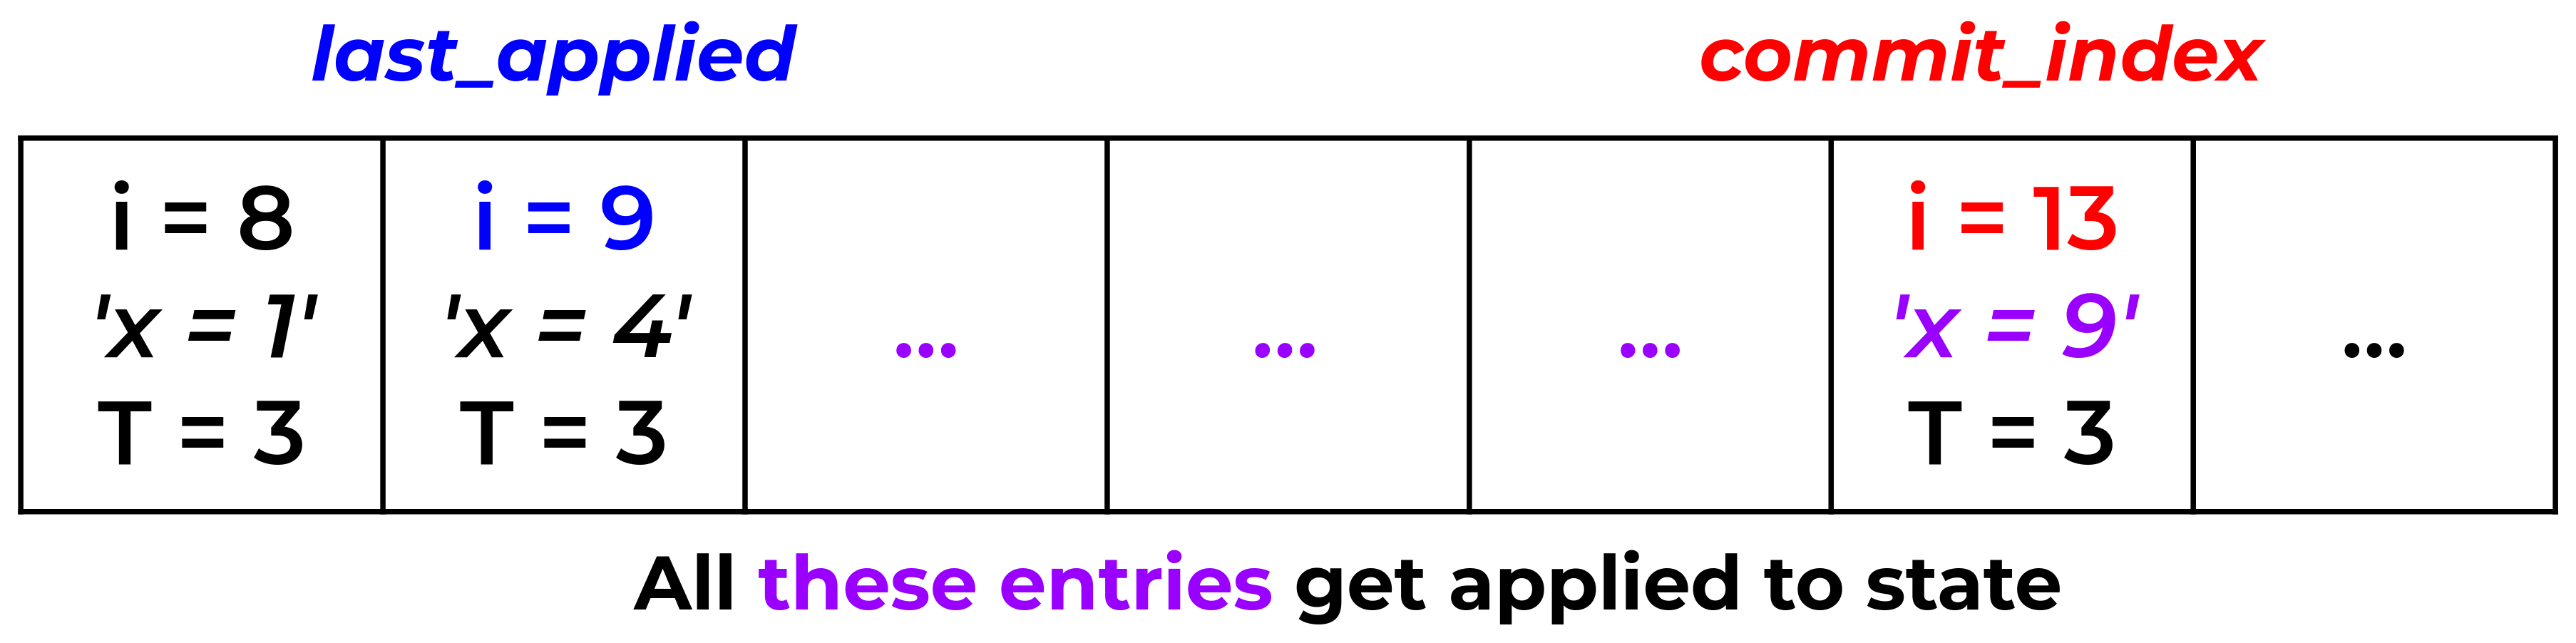
\includegraphics[width=.8\linewidth]{images/applyToState.png}
  
  \caption{All entries between \textit{last\_applied} and \textit{commit\_index} (included) get applied to state.}
  \Description{An array showing that all entries between the last applied and the last committed get applied to state.}
  \label{fig:applyToState}
\end{figure}

\begin{python}[label={code:applyToState}, caption={All nodes apply entries to state based on \textit{commit\_index}}]
def service_actions(self):
        # ...
        if self.commit_index is not None and self.commit_index > self.last_applied:   
            global raft_orders  # applying means appending entries to this queue

            #...

            last_applied_log_position: int = -1 
            for i, my_entry in enumerate(self.log):
                if (my_entry.index == self.last_applied):
                    last_applied_log_position = i
                    break # found log position of last applied entry 
            
            log_iterator = last_applied_log_position + 1    # improves code clarity 

            while self.last_applied != self.commit_index:
                raft_orders.put(self.log[log_iterator])
                self.last_applied = self.log[log_iterator].index
                log_iterator = log_iterator + 1
            # here self.last_applied == self.commit_index
\end{python}

\subsection{Log Compaction}

\subsection{Leader Election}

\subsection{Cluster Membership Change}

\subsection{Byzantine Raft}